\documentclass[reqno,a4paper,12pt]{amsart}

\usepackage{amsmath,amssymb,amsthm,geometry,xcolor,soul,graphicx}
\usepackage{titlesec}
%\usepackage{enumitem}
\usepackage{enumerate}
\usepackage{lipsum}
\usepackage{listings}
\allowdisplaybreaks[4] %align公式跨页
\RequirePackage[most]{tcolorbox}
\usepackage{braket}
%\usepackage{esint} %$\varoiint$ (带圈的二重积分)
%\usepackage[colorlinks,linkcolor=red]{hyperref} %\url{}超链接
\usepackage[scheme=plain,linespread=1,punct=CCT]{ctex}% Chinese support, single line space, narrow-version SBC case punctuations
\setCJKfamilyfont{zhsong}[AutoFakeBold={2.17}]{SimSong-Regular}
\renewcommand{\songti}{\CJKfamily{zhsong}}
%\usepackage{xeCJK}
%\setCJKmainfont{Kai}
\geometry{left=0.7in, right=0.7in, top=1in, bottom=1in}

\renewcommand{\baselinestretch}{1.3}

\title{固体物理第八次作业}
\author{董建宇 ~~ 2019511017}

\begin{document}

\maketitle
\titleformat{\section}[hang]{\small}{\thesection}{0.8em}{}{}
\titleformat{\subsection}[hang]{\small}{\thesubsection}{0.8em}{}{}

\section{\textbf{(13.1) Reciprocal Lattice}\\
Show that the reciprocal lattice of a fcc lattice is a bcc lattice. Correspondingly, show that the reciprocal lattice of a bcc lattice is an fcee lattice. If an fcc lattice has conventional unit cell with lattice constant $a$, what is the lattice constant for the conventional unit cell of the reciprocal bcc lattice? Consider now an orthorhombic face-centered lattice with conventional lattice constants $a_1, a_2, a_3$. What it the reciprocal lattice now?
}
\begin{tcolorbox}[breakable, colback = black!5!white, colframe = black]
考虑晶格常数为$a$的面心立方晶格,三个晶格基矢为:
\[
	\vec{a}_1 = \left( \frac{a}{2}, \frac{a}{2}, 0 \right), ~ \vec{a}_2 = \left( \frac{a}{2}, 0, \frac{a}{2} \right), ~ \vec{a}_3 = \left( 0, \frac{a}{2}, \frac{a}{2} \right).
\]
则倒空间中三个晶格基矢分别为:
\begin{align*}
	\vec{b}_1 =& \frac{2\pi (\vec{a}_2 \times \vec{a}_3)}{\vec{a}_1\cdot (\vec{a}_2\times\vec{a}_3)} = \left( \frac{2\pi}{a}, \frac{2\pi}{a}, -\frac{2\pi}{a} \right), \\
	\vec{b}_2 =& \frac{2\pi (\vec{a}_3 \times \vec{a}_1)}{\vec{a}_1\cdot (\vec{a}_2\times\vec{a}_3)} = \left( \frac{2\pi}{a}, -\frac{2\pi}{a}, \frac{2\pi}{a} \right), \\
	\vec{b}_3 =& \frac{2\pi (\vec{a}_1 \times \vec{a}_2)}{\vec{a}_1\cdot (\vec{a}_2\times\vec{a}_3)} = \left( -\frac{2\pi}{a}, \frac{2\pi}{a}, \frac{2\pi}{a} \right). 
\end{align*}
即倒空间中为体心立方晶格。 \\
考虑晶格常数为$b$的体心立方晶格,三个晶格基矢为:
\[
	\vec{a}_1' = \left( \frac{b}{2}, \frac{b}{2}, -\frac{b}{2} \right), ~ \vec{a}_2' = \left( \frac{b}{2}, -\frac{b}{2}, \frac{b}{2} \right), ~ \vec{a}_3' = \left( -\frac{b}{2}, \frac{b}{2}, \frac{b}{2} \right).
\]
则倒空间中三个晶格基矢分别为:
\begin{align*}
	\vec{b}_1' =& \frac{2\pi (\vec{a}_2' \times \vec{a}_3')}{\vec{a}_1'\cdot (\vec{a}_2'\times\vec{a}_3')} = \left( \frac{2\pi}{b}, \frac{2\pi}{b}, 0 \right), \\
	\vec{b}_2' =& \frac{2\pi (\vec{a}_3' \times \vec{a}_1')}{\vec{a}_1'\cdot (\vec{a}_2'\times\vec{a}_3')} = \left( \frac{2\pi}{b}, 0, \frac{2\pi}{b} \right), \\
	\vec{b}_3' =& \frac{2\pi (\vec{a}_1' \times \vec{a}_2')}{\vec{a}_1'\cdot (\vec{a}_2'\times\vec{a}_3')} = \left( 0, \frac{2\pi}{b}, \frac{2\pi}{b} \right). 
\end{align*}
即倒空间中为面立方晶格。 \\
设fcc晶格对应的倒空间中bcc晶格常数为$l$,由上述分析可知:
\[
	\frac{2\pi}{a} = \frac{l}{2}.
\]
即倒空间中bcc晶格的晶格常数为$l = \frac{4\pi}{a}$。 \\
对于一个面心正交晶格,晶格常数为$a_1, a_2, a_3$,晶格基矢为:
\[
	\vec{v}_1 = \left( \frac{a_1}{2}, \frac{a_2}{2}, 0 \right), ~ \vec{v}_2 = \left( \frac{a_1}{2}, 0, \frac{a_3}{2} \right), ~ \vec{v}_3 = \left( 0, \frac{a_2}{2}, \frac{a_3}{2} \right).
\]
在倒空间中晶格基矢分别为:
\begin{align*}
	\vec{u}_1 =& \frac{2\pi(\vec{v}_2 \times \vec{v}_3)}{\vec{v}_1 \cdot (\vec{v}_2\times\vec{v}_3)} = \left( \frac{2\pi}{a_1}, \frac{2\pi}{a_2}, -\frac{2\pi}{a_3} \right), \\
	\vec{u}_2 =& \frac{2\pi(\vec{v}_3 \times \vec{v}_1)}{\vec{v}_1 \cdot (\vec{v}_2\times\vec{v}_3)} = \left( \frac{2\pi}{a_1}, -\frac{2\pi}{a_2}, \frac{2\pi}{a_3} \right), \\
	\vec{u}_3 =& \frac{2\pi(\vec{v}_1 \times \vec{v}_2)}{\vec{v}_1 \cdot (\vec{v}_2\times\vec{v}_3)} = \left( -\frac{2\pi}{a_1}, \frac{2\pi}{a_2}, \frac{2\pi}{a_3} \right).
\end{align*}
即在倒空间中为体心正交晶格,晶格常数为$\frac{4\pi}{a_1}, \frac{4\pi}{a_2}, \frac{4\pi}{a_3}$.
\end{tcolorbox}

\section{\textbf{(13.2) Lattice Planes} \\
Consider the crystal shown in Exercise 12.3. Copy this figure and indicate the [210] direction and the (210) family of lattice planes.
}
\begin{tcolorbox}[breakable, colback = black!5!white, colframe = black]
习题12.3中晶格为面心立方结构,基元为位于(0,0,0)的锌原子与(0.25,0.25,0.75)的硫原子。当常规晶格的晶格常数为$a$时,晶格基矢为:
\[
	\vec{a}_1 = \left( \frac{a}{2}, \frac{a}{2}, 0 \right), ~ \vec{a}_2 = \left( \frac{a}{2}, 0, \frac{a}{2} \right), ~ \vec{a}_3 = \left( 0, \frac{a}{2}, \frac{a}{2} \right).
\]
在实空间中,晶格平面满足(1/2,1,0),即下图:\\
\begin{centering}
	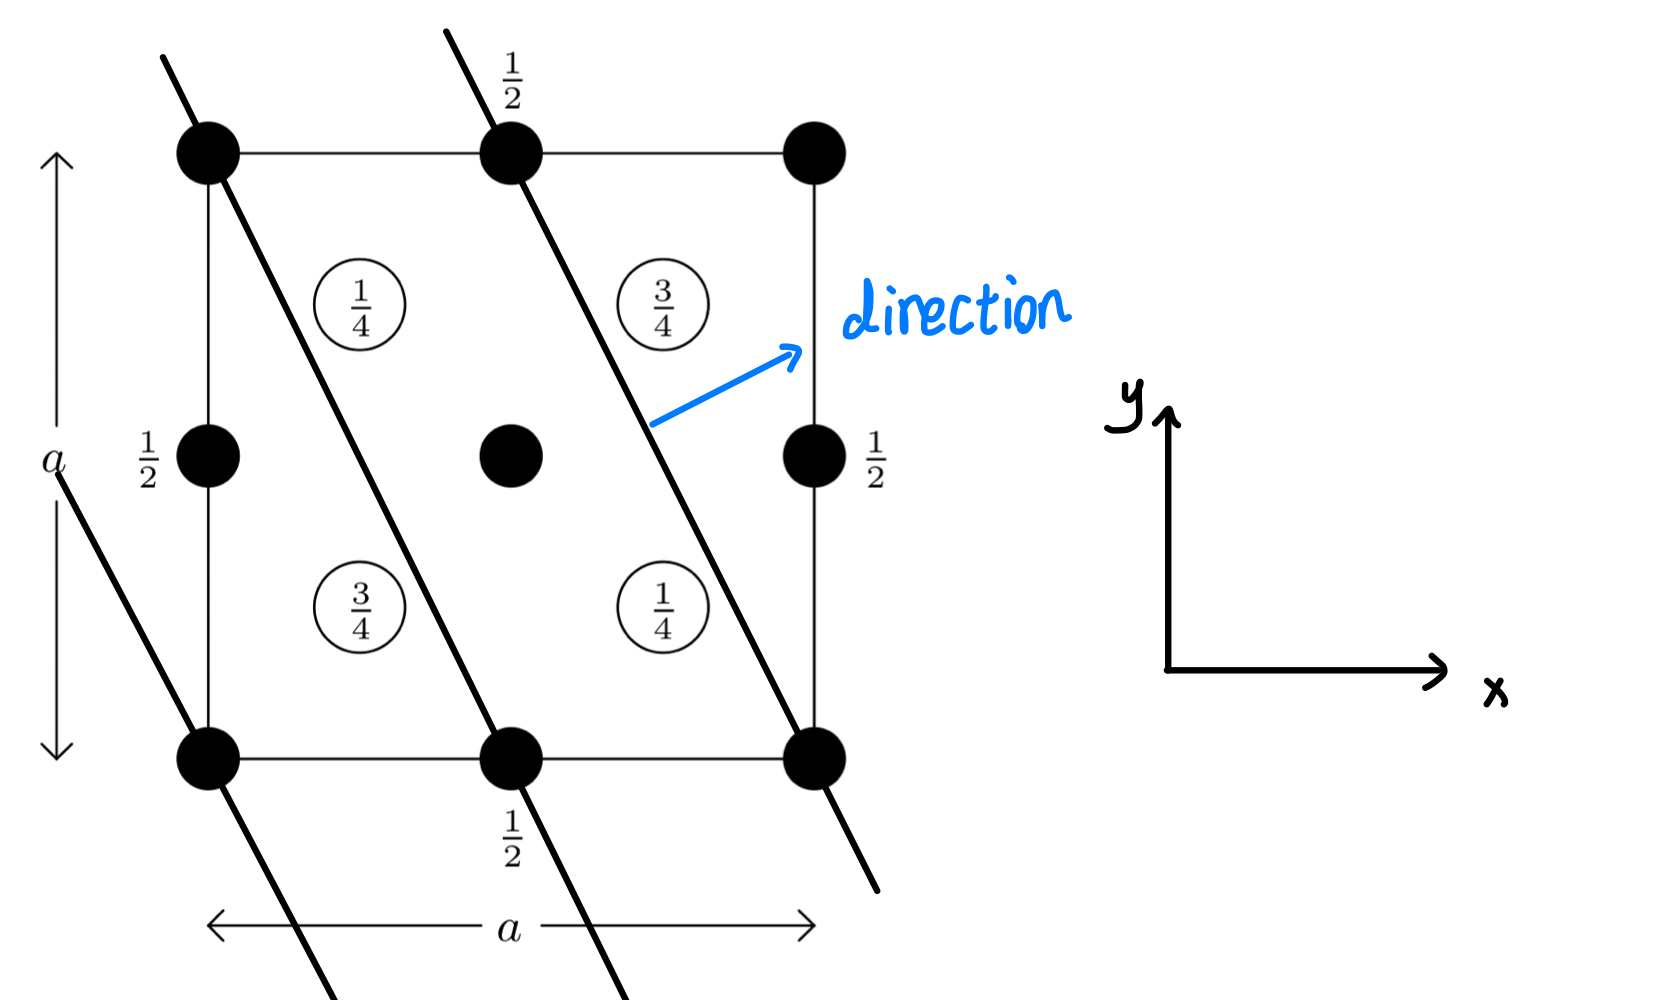
\includegraphics[scale = 0.2]{13.2.jpeg}
\end{centering} \\
蓝色箭头表示方向矢量,此图为z轴俯视图(忽略途中表示z轴方向高度)。从图中可以注意到有些原子并未包含在这组平面(2x+y = ma)内,但是若Miller指数写为(4,2,0)则晶格平面为(4x+2y = ma)包含了所有的原子。其中m为整数。
%则在倒空间中基矢为:
%\begin{align*}
%	\vec{b}_1 =& \frac{2\pi (\vec{a}_2 \times \vec{a}_3)}{\vec{a}_1\cdot (\vec{a}_2\times\vec{a}_3)} = \left( \frac{2\pi}{a}, \frac{2\pi}{a}, -\frac{2\pi}{a} \right), \\
%	\vec{b}_2 =& \frac{2\pi (\vec{a}_3 \times \vec{a}_1)}{\vec{a}_1\cdot (\vec{a}_2\times\vec{a}_3)} = \left( \frac{2\pi}{a}, -\frac{2\pi}{a}, \frac{2\pi}{a} \right), \\
%	\vec{b}_3 =& \frac{2\pi (\vec{a}_1 \times \vec{a}_2)}{\vec{a}_1\cdot (\vec{a}_2\times\vec{a}_3)} = \left( -\frac{2\pi}{a}, \frac{2\pi}{a}, \frac{2\pi}{a} \right). 
%\end{align*}
%则[210]矢量为:
%\[
%	\vec{G}_{(2,1,0)} = 2\vec{b}_1 + \vec{b}_2 = \left( \frac{6\pi}{a}, \frac{2\pi}{a}, -\frac{2\pi}{a} \right)
%\]
%方向(单位矢量)为:
%\[
%	\vec{u}_{(2,1,0)} = \frac{\vec{G}_{(2,1,0)}}{\vert \vec{G}_{(2,1,0)} \vert} = \left( \frac{3}{\sqrt{11}}, \frac{1}{\sqrt{11}}, -\frac{1}{\sqrt{11}} \right).
%\]
%晶格平面族满足:
%\[
%	\vec{r} \cdot \vec{G}_{(2,1,0)} = 2\pi m,
%\]
%其中$m\in Z$,令$\vec{r} = (x,y,z)$,则晶格平面族为:
%\[
%	3x+y-z = ma.
%\]
%其中$m\in Z$。
\end{tcolorbox}

\section{\textbf{(13.3) Directions and Spacings of Crystal Planes}\\
$\triangleright ~~ \ddagger$ Explain briefly what is meant by the terms "crystal planes" and "Miller indices". \\
$\triangleright$ Show that the general direction $[hkl]$ in a cubic crystal is normal to the planes with Miller indices (hkl). \\
$\triangleright$ Is the same true in general for an orthorhombic crystal? \\
$\triangleright$ Show that the spacing $d$ of the $(hkl)$ set of planes in a cubic crystal with lattice parameter $a$ is 
\[
	d = \frac{a}{\sqrt{h^2+k^2+l^2}}
\]
$\triangleright$ What is the generalization of this formula for an orthorhombic crystal?
}
\begin{tcolorbox}[breakable, colback = black!5!white, colframe = black]
$\triangleright$晶格平面是一些由晶体中三个不共线的点组成的一系列平行的平面。Miller指数是一个包含三个整数元素的集合,确定一组互相平行的晶格平面。 \\
$\triangleright$在给定Miller指数(hkl)条件下,实空间中$(1/h, 0, 0), (0, 1/k, 0), (0, 0, 1/l)$为实空间中距原点最近的晶格平面,则该平面上任意一点可以写为:
\[
	\alpha \left( \frac{\vec{a}_1}{h} - \frac{\vec{a}_2}{k} \right) + \beta \left( \frac{\vec{a}_1}{h} - \frac{\vec{a}_3}{l} \right).
\]
则可以计算:
\[
	(h\vec{a}_1 + k\vec{a}_2 + l\vec{a}_3)\left( \alpha \left( \frac{\vec{a}_1}{h} - \frac{\vec{a}_2}{k} \right) + \beta \left( \frac{\vec{a}_1}{h} - \frac{\vec{a}_3}{l} \right) \right) = \alpha a^2 - \alpha a^2 + \beta a^2 - \beta a^2 = 0.
\]
其中晶格矢量点乘满足:
\[
	\vec{a}_i \cdot \vec{a}_j = a^2\delta_{ij}.
\]
$\triangleright$在正交晶系中,各个晶格矢量仍满足正交关系,但各自的模长不同,再次计算可得:
\[
	(h\vec{a}_1 + k\vec{a}_2 + l\vec{a}_3)\left( \alpha \left( \frac{\vec{a}_1}{h} - \frac{\vec{a}_2}{k} \right) + \beta \left( \frac{\vec{a}_1}{h} - \frac{\vec{a}_3}{l} \right) \right) = \alpha (a_1^2 - a_2^2) + \beta (a_1^2 - a_3^2).
\]
不恒等于0,即对于正交晶系,常规方向[hkl]与Miller指数(hkl)确定的方向并不一定垂直。 \\
$\triangleright$对于Miller指数(hkl)的晶格平面,倒格矢为:
\[
	\vec{G} = h\vec{b}_1 + k\vec{b}_2 + l\vec{b}_3.
\]
其中,
\[
\vert \vec{b}_1 \vert = \vert \vec{b}_2 \vert = \vert \vec{b}_3 \vert = \frac{2\pi}{a}
\]
晶格平面间距为:
\[
	d = \frac{2\pi}{\vert \vec{G} \vert} = \frac{2\pi}{\sqrt{(h^2+k^2+l^2)\frac{4\pi^2}{a^2}}} = \frac{a}{\sqrt{h^2+k^2+l^2}}. 
\]
$\triangleright$对于正交晶系,各个晶格矢量满足正交关系,但各自模长不同,则有:
\[
	\vert \vec{b}_i \vert = \frac{2\pi}{a_i}.
\]
其中$a_i$表示i方向晶格常数。 \\
当Miller指数为(hkl)时,晶格平面间距为:
\[
	d = \frac{2\pi}{\vert \vec{G} \vert} = \frac{2\pi}{\sqrt{4\pi^2 \left( \frac{h^2}{a_1^2} + \frac{k^2}{a_2^2} + \frac{l^2}{a_3^2} \right)}} = \frac{1}{\sqrt{\frac{h^2}{a_1^2} + \frac{k^2}{a_2^2} + \frac{l^2}{a_3^2}}}.
\]
\end{tcolorbox}

\section{\textbf{(13.4) $\ddagger$ Reciprocal Lattice} \\
(a) Define the term Reciprocal Lattice. \\
(b) Show that if a lattice in 3d has primitive lattice vectors $\vec{a}_1$, $\vec{a}_2$ and $\vec{a}_3$ then primitive lattice vectors for the reciprocal lattice can be taken as 
\begin{align*}
	\vec{b}_1 =& \frac{2\pi (\vec{a}_2 \times \vec{a}_3)}{\vec{a}_1\cdot (\vec{a}_2\times\vec{a}_3)}, \\
	\vec{b}_2 =& \frac{2\pi (\vec{a}_3 \times \vec{a}_1)}{\vec{a}_1\cdot (\vec{a}_2\times\vec{a}_3)}, \\
	\vec{b}_3 =& \frac{2\pi (\vec{a}_1 \times \vec{a}_2)}{\vec{a}_1\cdot (\vec{a}_2\times\vec{a}_3)}. 
\end{align*}
What is the proper formula in 2d? \\
(c) Define tetragonal and orthorhombic lattice. For an orthorhombic lattice, show that $\vert \vec{b}_j \vert = \frac{2\pi}{\vert \vec{a}_j \vert}$. Hence, show that the length of the reciprocal lattice vector $\vec{G} = h\vec{b}_1 + k\vec{b}_2 + l\vec{b}_3$ is equal to $2\pi/d$, where $d$ is the spacing of the $(hkl)$ planes (see equation 13.3)
}
\begin{tcolorbox}[breakable, colback = black!5!white, colframe = black]
\begin{enumerate}[(a)]
\item 倒格子中格点矢量$\vec{k}$满足以下条件:
\[
	\vec{k} \cdot \vec{R} = 2m\pi.
\]
其中$\vec{R}$为实空间中格点矢量,$m$为整数。 \\
\item 可以计算:
\begin{align*}
	\vec{a}_1 \cdot \vec{b}_1 &= \frac{2\pi \vec{a}_1 \cdot (\vec{a}_2\times\vec{a}_3)}{\vec{a}_1 \cdot (\vec{a}_2\times\vec{a}_3)} = 2\pi; \\
	\vec{a}_2 \cdot \vec{b}_2 &= \frac{2\pi \vec{a}_2 \cdot (\vec{a}_3\times\vec{a}_1)}{\vec{a}_1 \cdot (\vec{a}_2\times\vec{a}_3)} = 2\pi; \\
	\vec{a}_3 \cdot \vec{b}_3 &= \frac{2\pi \vec{a}_3 \cdot (\vec{a}_1\times\vec{a}_2)}{\vec{a}_1 \cdot (\vec{a}_2\times\vec{a}_3)} = 2\pi.
\end{align*}
对于$i\neq j$,可以计算:
\[
	\vec{a}_i \cdot \vec{b}_j = 0.
\]
综上所述,有:
\[
	\vec{a}_i \cdot \vec{b}_j = 2\pi \delta_{ij}.
\]
对于二维晶格,只需要取$\vec{a}_3$为垂直于平面的单位向量$\hat{e}_z$,然后可以计算二维倒格矢:
\begin{align*}
	\vec{b}_1 &= \frac{2\pi(\vec{a}_2 \times \hat{e}_z)}{\vec{a}_1\cdot (\vec{a}_2 \times \hat{e}_z)}; \\
	\vec{b}_2 &= \frac{2\pi(\hat{e}_z \times \hat{a}_1)}{\vec{a}_1\cdot (\vec{a}_2 \times \hat{e}_z)}.
\end{align*}
\item 对于四方晶系,晶格常数满足:$a_1 = a_2 \neq a_3$, $\alpha = \beta = \gamma = \frac{\pi}{2}$. \\
对于立方晶系,晶格常数满足:$a_1 \neq a_2 \neq a_3$, $\alpha = \beta = \gamma = \frac{\pi}{2}$. \\
对于立方晶系,由于任意两个晶格矢量间夹角均为$\frac{\pi}{2}$,则有:
\[
	\vec{a}_i \times \vec{a}_j = \sum_k\epsilon_{ijk} \vert \vec{a}_i \vert \vert \vec{a}_j \vert \hat{e}_k
\]
其中$\hat{e}_k$为沿$\vec{a}_k$方向的单位矢量。则可以计算得:
\begin{align*}
	\vert \vec{b}_1 \vert &= 2\pi \frac{\vert \vec{a}_2\times\vec{a}_3 \vert}{\vert \vec{a}_1 \vert \vert \vec{a}_2\times\vec{a}_3 \vert} = \frac{2\pi}{\vert \vec{a}_1 \vert}; \\
	\vert \vec{b}_2 \vert &= 2\pi \frac{\vert \vec{a}_3\times\vec{a}_1 \vert}{\vert \vec{a}_1 \vert \vert \vec{a}_2\times\vec{a}_3 \vert} = 2\pi\frac{\vert \vec{a}_3\times\vec{a}_1 \vert}{\vert \vec{a_2} \vert \vert \vec{a}_3 \times \vec{a}_1 \vert} = \frac{2\pi}{\vert \vec{a}_2 \vert}; \\
	\vert \vec{b}_3 \vert &= 2\pi \frac{\vert \vec{a}_1\times\vec{a}_2 \vert}{\vert \vec{a}_1 \vert \vert \vec{a}_2\times\vec{a}_3 \vert} = 2\pi\frac{\vert \vec{a}_1\times\vec{a}_2 \vert}{\vert \vec{a}_3 \vert \vert \vec{a}_1 \times \vec{a}_2 \vert} = \frac{2\pi}{\vert \vec{a}_3 \vert}.
\end{align*}
综上,有:
\[
	\vert \vec{b}_j \vert = \frac{2\pi}{\vert \vec{a}_j \vert}.
\]
倒格矢长度为:
\[
	\vert \vec{G} \vert = \sqrt{h^2 \vert \vec{b}_1 \vert^2 + k^2 \vert \vec{b}_2 \vert^2 + l^2 \vert \vec{b}_3 \vert^2} = 2\pi\sqrt{\frac{h^2}{a_1^2} + \frac{k^2}{a_2^2} + \frac{l^2}{a_3^2}} = \frac{2\pi}{d}.
\]
\end{enumerate}
\end{tcolorbox}

\section{\textbf{(13.5) More Reciprocal Lattice} \\
A two-dimensional rectangular crystal has a unit cell with sides $a_1 = 0.468$nm and $a_2 = 0.342$nm. \\
(a) Draw to scale a diagram of the reciprocal lattice. \\
$\triangleright$ Label the reciprocal lattice points for indices in the range $0 \leq h \leq 3$ and $0 \leq k \leq 3$. \\
(b) Draw the first and second Brillouin zones using the Wigner-Seitz construction. 
}
\begin{tcolorbox}[breakable, colback = black!5!white, colframe = black]
\begin{enumerate}[(a)]
\item 在倒空间中,晶格常数分别为:
\[
	b_1 = \frac{2\pi}{a_1} \approx 13.4nm^{-1}, ~~ b_2 = \frac{2\pi}{a_2} \approx 18.4 nm^{-1}.
\]
其中格点指数在$0\leq h \leq 3$及$0\leq k\leq 3$范围内的格点在图中标出。 \\
\item 图中蓝色阴影区域表示第一布里渊区,红色阴影区域表示第二部里渊区。 \\
\begin{centering}
	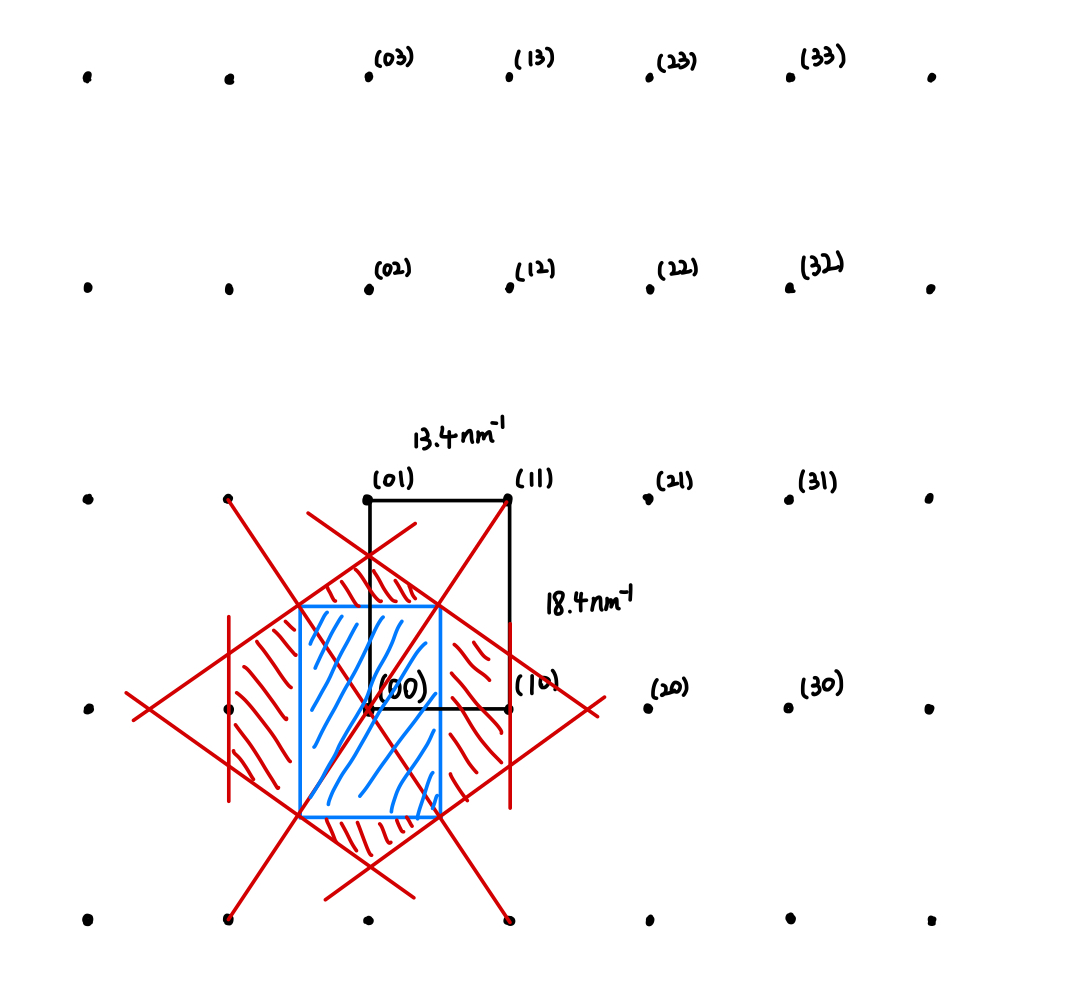
\includegraphics[scale = 0.192]{13.5.jpeg}
\end{centering}
\end{enumerate}
\end{tcolorbox}

\section{\textbf{(13.6) Brillouin Zones} \\
(b) Consider a triangular lattice in two dimensions (primitive lattice vectors given by Eqs. 12.3). Find the first Brillouin zone. Given an arbitrary wavevector $\mathbf{k}$ (in two dimensions), write an expression for an equivalent wavevector within the first Brillouin zone (again there are several possible expression you can write).
}
\begin{tcolorbox}[breakable, colback = black!5!white, colframe = black]
实空间中两个基矢为:
\[
	\vec{a}_1 = a\hat{x}, ~~ \vec{a}_2 = (a/2)\hat{x} + (a\sqrt{3}/2)\hat{y}.
\]
则可以计算在倒空间中基矢为:
\begin{align*}
	\vec{b}_1 &= 2\pi \frac{\vec{a}_2 \times \hat{z}}{\vec{a}_1\cdot (\vec{a}_2 \times \hat{z})} = \frac{2\pi}{a} \left( \hat{x} - \frac{1}{\sqrt{3}}\hat{y} \right), \\
	\vec{b}_2 &= 2\pi \frac{\hat{z} \times \vec{a}_1}{\vec{a}_1\cdot (\vec{a}_2 \times \hat{z})} = \frac{2\pi}{a} \frac{2}{\sqrt{3}}\hat{y}.
\end{align*}
注意到:
\[
	\vert \vec{b}_1 \vert = \vert \vec{b}_2 \vert = \frac{4\pi}{\sqrt{3}a}.
\]
绘制倒空间晶格如下:其中蓝色阴影区域和红色阴影区域分别为不同形式的的第一布里渊区。 \\
\begin{centering}
	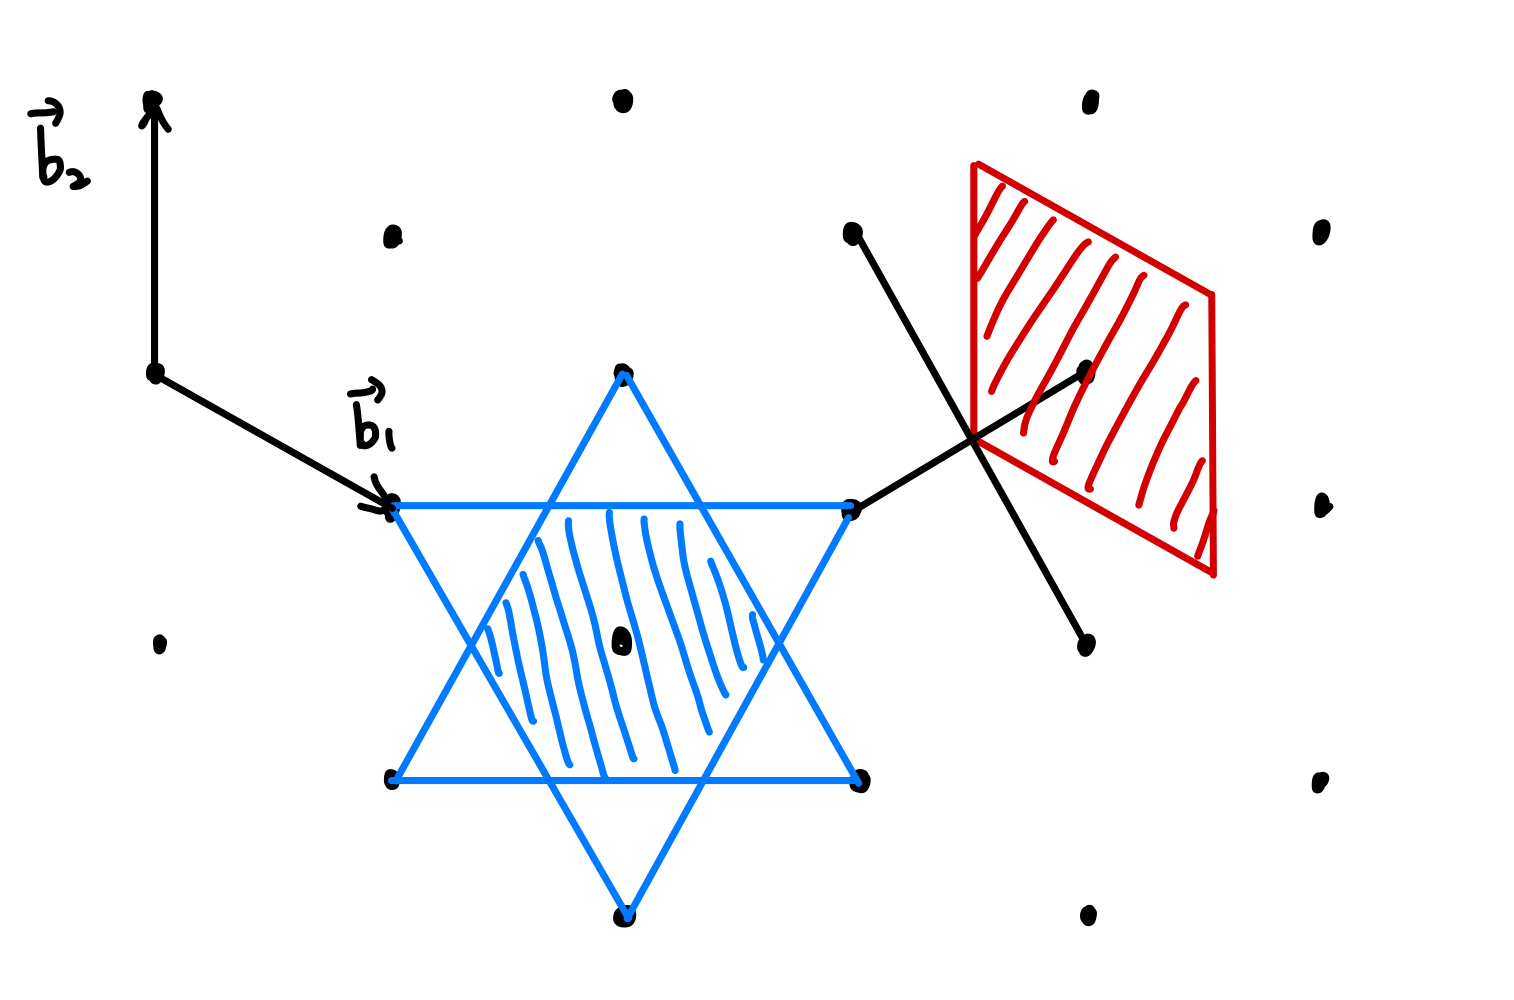
\includegraphics[scale = 0.14]{13.6.jpeg}
\end{centering} \\
在倒空间中任意一个波矢都可以写成两个基矢的线性组合,即
\[
	\vec{k} = m \vec{b}_1 + n \vec{b}_2.
\]
可以计算:
\begin{align*}
	\vec{k} \cdot \vec{b}_1 &= m \vert \vec{b}_1 \vert^2 + n \vec{b}_2 \cdot \vec{b}_1 = \frac{8\pi^2}{3a^2}(2m-n), \\
	\vec{k} \cdot \vec{b}_2 &= m \vec{b}_1 \cdot \vec{b}_2 + n\vert \vec{b}_2 \vert^2 = \frac{8\pi^2}{3a^2}(2n-m).
\end{align*}
则可以解得:
\begin{align*}
	m =& \frac{a^2}{8\pi^2}(2\vec{k} \cdot \vec{b}_1 + \vec{k} \cdot \vec{b}_2), \\
	n =& \frac{a^2}{8\pi^2}(\vec{k} \cdot \vec{b}_1 + 2\vec{k} \cdot \vec{b}_2).
\end{align*}
考虑上图中红色阴影区域的第一布里渊区,则该区域中任意一点的波矢可以写为:
\[
	\vec{k}' = \alpha \vec{b}_1 + \beta \vec{b}_2,
\]
其中$\alpha, \beta \in [-1/2, 1/2]$。可以令
\begin{align*}
	m' =& m - \lfloor m+0.5 \rfloor, \\
	n' =& n - \lfloor n+0.5 \rfloor.
\end{align*}
可以验证:$m', n' \in [-1/2, 1/2]$。即在第一布里渊区的等效波矢为:
\[
	\vec{k}_0 = (m - \lfloor m+0.5 \rfloor) \vec{b}_1 + (n - \lfloor n+0.5 \rfloor) \vec{b}_2.
\]
其中$\lfloor x \rfloor$表示对x向下取整。
\end{tcolorbox}

\section{\textbf{(13.7) Number of States in the Brillouin Zone} \\
A specimen in the form of a cube of side $L$ has a primitive cubic lattice whose mutually orthogonal fundamental translation vectors (primitive lattice vectors) have length $a$. Show that the number of different allowed \textbf{k-}states within the first Brillouin zone equals the number of primitive unit cells forming the specimen. (One may assume periodic boundary conditions, although it is worth thinking about whether this still holds for hard-wall boundary conditions as well.)
}
\begin{tcolorbox}[breakable, colback = black!5!white, colframe = black]
考虑周期性边界条件:
\[
	e^{ik_x(x+L)} = e^{ikx}.
\]
则有在倒空间中$k_x$的可能取值为:
\[
	k_x = h\frac{2\pi}{L},
\]
其中$h$为整数,同理可以计算$k_y$和$k_z$的可能取值:
\[
	\vec{k} = (h,k,l)\frac{2\pi}{L}.
\]
则在倒空间中,每一个态占据空间大小为$\frac{8\pi^3}{L^3}$。第一布里渊区的体积为$\frac{8\pi^3}{a^3}$。则在第一布里渊区中允许的态的数目为:
\[
	N_1 = \frac{\frac{8\pi^3}{a^3}}{\frac{8\pi^3}{L^3}} = \frac{L^3}{a^3}.
\]
体系中原初晶包的个数为:
\[
	N_2 = \frac{L^3}{a^3} = N_1.
\]
即第一布里渊区允许的态数目等于体系包含的原初晶包数目。
\end{tcolorbox}

\end{document}